\section{Discussion}
% 1 page
To be done...

- Estimates was largely correct, although we had forgotten some tasks

- Incorrect server behavior which could not be foreseen occurred, which slowed our progress down. This is the faults from the first part of the project which haunts us.

- Capability Maturity Model improvement

- How well did we manage to rescue the project as seen from the current state of the project? Do it seem like we are succeeding? The report needs much work, we are barely started.

The Capability Maturity Model, created by the Software Engineering Institute of Carnegie Mellon University, describes the development process an organization must pass through to be considered mature.
 
 \begin{figure}[t]
  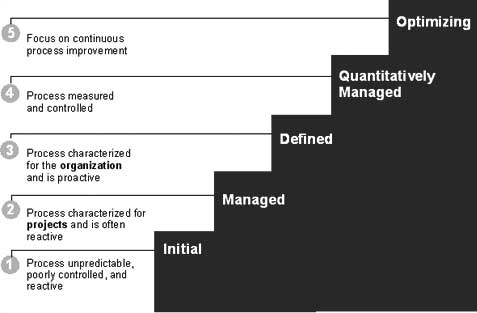
\includegraphics[width=\textwidth]{illustrations/CMM.jpg}
  \caption{Capability Maturity Model. Source: [\textit{http://www.tutorialspoint.com/cmmi/cmmi-maturity-levels.htm}]}
  \label{fig:Capability_Maturity_Model}
\end{figure}

While doing our project, we moved from the initial level of the Capability Maturity Model (while developing the server) to the managed level (during the development of the client) \cite[p. 242]{PM}. We kept to the initial level during the development of the server, by developing as we went along without using well known development methods or initial design (see figure \ref{fig:Capability_Maturity_Model}). It illuminates exactly what we want to show in this report, that using many of these tools gives us a huge advantage of producing a product, while not using any of these tools it is very uncertain any useful product can be made.

CISQ, the Consortium for IT Software Quality, is comprised by people from different parts of the software industry. It is a neutral forum for customers and suppliers of IT to define, measure and improve IT quality.

If the product fulfills the requirements and pass the tests, its \textbf{reliability} has been proved as well, which is one of CISQ's  major desirable characteristics. The other 4 are; efficiency, security, maintainability and size \cite{CISQ}

\textbf{[ TODO: Update the source if its still is needed once this has been rewritten. ]}

\begin{itemize}
	\item Efficiency means that there is minimal to none code duplication, the algorithms are optimized, etc. The code runs as smooth and fast as possible at production.
	\item Security is about how vulnerable the code is to direct attacks. If there are any obvious breaches then they affect this criteria.
	\item Maintainability: How easy is it to understand and edit the product once in production. Documented code and the clear use of known design patterns increases maintainability. 
	\item Size is not a quality indicator per see, but can be used to asses the time needed to complete the product.
\end{itemize}

How our project is measured on these five characteristics:
\begin{itemize}
 	\item The reliability of our server have been a main focus of the group. The server will continue to run after most exceptions, though the server host has been unstable and have had some irregular uptime.
 	\item The efficiency parameter comes partly from our planning and software design and partly from our implementation. This where our client differ from our server thanks to the tools we chose to use, the efficiency of the server is determined by what we found worked while coding it.
 	\item We have not prioritized security, the server does not encrypt anything. Nor is the connection between the server and client encrypted. We have deliberately chosen this as we found other elements such as streaming, more important. We acknowledge this as unacceptable if it was an actual product.  
 	\item The client is maintainable: We have a well documented and responsibility-driven product, making it easy for others to understand and maintain our code. The server is documented as well, but it is not as transparent as the client.
	\item Size can be used to determine whether we have made it too complicated. If we, from the beginning, had made interfaces for all the modules of our server, we would have seen an overly complex system, but we only discovered this after the server was almost completed. While our client seems large it is a conscious choice to lessen the complexity of the individual classes.  
\end{itemize}
\newpage